This chapter provides important artifacts related to design of our project.

\section{Software Design}

This is a class UML Diagram which contain classes of the main actors alongside their attributes and their behaviors. There are 11 classes each having their own specific attributes and functions clearly defining the flow and functionality of the system.
\subsection{Classes}
\begin{enumerate}
    \item  User
    \item  Jobs
    \item  Routes
    \item  BaseUser
    \item  Sessions
    \item  Admin
    \item  Location
    \item  Images
    \item  Pre-Processing  (Static Class)
    \item GarbNetModel    (Static Class)
    \item Quantification  (Static Class)

\end{enumerate}


\newpage
\begin{figure}[!hb]
   \centering
   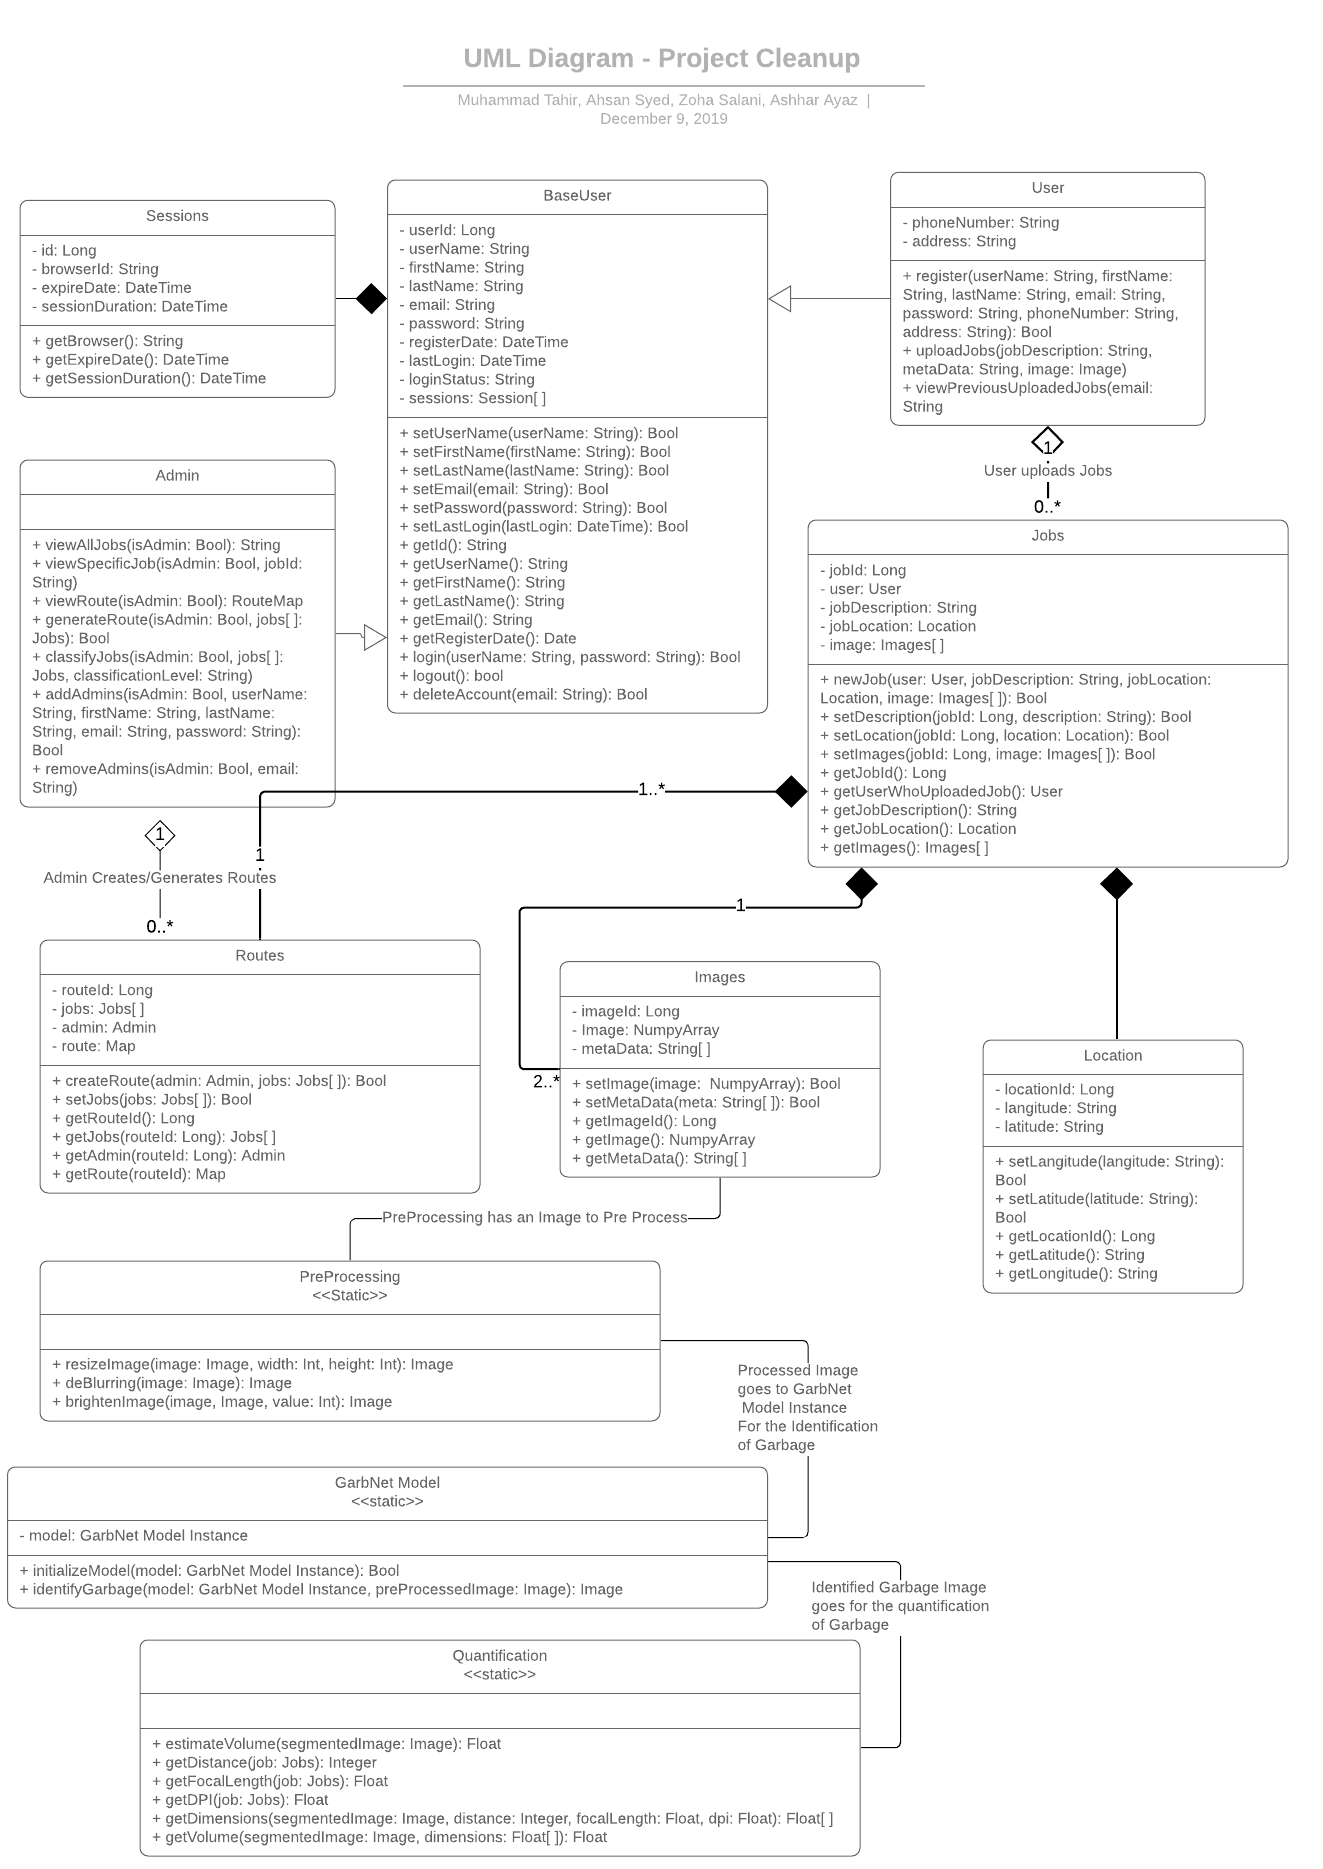
\includegraphics[scale=0.6]{images/UML.png}
   \caption{UML Diagram}\label{fig:picture}
\end{figure}

\subsection{UML Description}
Base User class refers to all the user classes that are accessing the system that is it includes both the User and the Admin but since they are separate entities (Actors) they will also have their own separate classes and will be inheriting from the parent class which in our case is the BaseUser. This particular class contains its particular attributes and functions that will remain the same for both the admin and the user entity. The relationship between the User class and the Admin class with the Base User is of generalization that is one element is a specialization of another general component. It may be substituted for it and is mostly used to represent inheritance. The Base User in this case is the Parent Class.\\
\\Now, Session Class having its defined attributes and functions is related to the BaseUser Class by the relation of Composition.The relationship is as such that if a composite object is deleted, all other objects associated with it are deleted. The composite object in this case is of the class BaseUser.\\
\\User Class having its own specific attributes and function is associated by aggregation relation with the Job Class that is a User can upload multiple Jobs. The relation is that of aggregation because the child class object can meaningfully, which in this case is Jobs, exist without the parent class object, unlike in composition.\\
\\Job Class having its specific attributes and functions is the composite for the Route, Images and Location Class that is if we delete the job, the route or image associated with that particular job will be deleted. The relationship is of composition.\\
\\Route Class is related to the admin by the relation of aggregation that is if we delete the admin the routes will still exist and if the Admin Class exist it can view all the routes generated.\\
\\The Image Class is associated with the the Pre-Processing Static Class as the latter accepts images and pre-processess. The Pre-Processed images are then passed into the GarbNet Model in order to identify garbage which is then passed to the Quantification Class. Here, the garbage is quantified, the volume is estimated and the value of Volume in Job class is updated for the Route Generation.


% Your report will contain ONE of the following 2 sections.
\newpage
\section{Data Design}

This section presents the structure of our database that caters to persistent data storage in our project. The structure is shown as a normalized data model for relational databases.
\subsection{ERD}
The ERD is the high-level conceptual diagram explaining the working of our project. This diagram shows the entities and the relationship of the entities stored in a database. The diagram will help explain the logical structure of the database.\\
\\The Entity Relationship Diagram for our database as follows:
\begin{figure}[!hb]
   \centering
   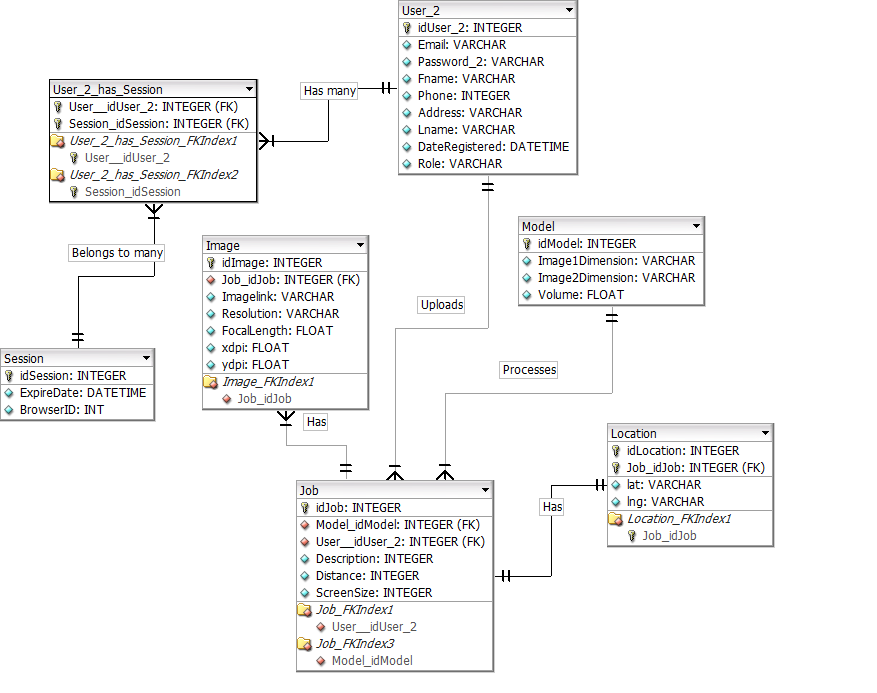
\includegraphics[scale=0.4]{images/ERD.png}
    \caption{Entity Relationship Diagram}\label{fig:picture}
\end{figure}
\newpage
Entities:\\
The strong entities in our relational diagram are as follows:\\
\textbf{1)User:}\\
\textbf{Primary Key:}UserID\\
\\
\textbf{2)Job:}\\
\textbf{Primary Key:} JobID\\
\textbf{Foreign Key:} AdminID\\
\textbf{Foreign Key:} UserID\\
\textbf{Foreign Key:} ModelID\\
\\
\textbf{3)Model:}\\
\textbf{Primary Key:} ModelID\\
\\
\textbf{3)Session:}\\
\textbf{Primary Key:} SessionID\\
\\
\textbf{4)Location:}\\
\textbf{Primary Key:} LocationID\\
\textbf{Foreign Key:} JobID\\
\\
\textbf{5)User has Session:}\\
\textbf{Primary Key:} UserID (FK)\\
\textbf{Primary Key:} SessionID (FK)\\
\\
\textbf{6)Admin:}\\
\textbf{Primary Key}: AdminID\\
\\
\textbf{7)Image:}\\
\textbf{Primary Key:} ImageID\\
\textbf{Foreign Key:} UserID\\
\\
Each entity has their own attributes that are specific to them. The entities also maintain a relationship between each other which is as follows:\\
\\
The User having login credentials and identifying fields, which are its specific attributes, is connected to the entity (Job) by a one to many relation that is one user can upload multiple jobs and can view the previous jobs. The User is also connected with the session entity which is a weak entity by a many to many relation since one session can have many users and one user can participate in various sessions.\\
\\
The Admin entity again with the login credentials and identifying fields is connected to the Job entity as one admin can view multiple jobs.\\
\\
The Model entity similarly is related to the Job entity by a many to one relationship as one model which exits for our application can process more than one jobs that are uploaded by the users.\\
\\
The Location Entity is related to the Job entity by a one to one relation since each Job will have a location of its own.\\
\\
Lastly, the image entity having its own attributes containing the image link and the image properties such as the resolution, focal length, location tag etc. is connected to the Job entity by having a one to may relation, that is a job can have multiple images but one specific image can belong to one and only one job only. The part where user can take multiple pictures is also catered as jobs contains the foreign key for the user entity.\\





 

